% =============================================================================
% Turkish translation of main.tex, for review only. The report that is submitted
% is main.tex. Sentences that the organisers' template fixes in English are
% translated here as well, so that the whole text can be read in one language.
% Same class, preamble, bibliography and figures as main.tex.
% =============================================================================

\documentclass[sigconf]{acmart}
% =============================================================================
% Template setup — participants normally do not edit this file.
% Author content belongs in main.tex; citations belong in main.bib.
% \documentclass lives in main.tex so Overleaf does not treat this file as root.
% =============================================================================

% --- Competition / non-ACM-submission friendly rights metadata -------------
\setcopyright{none}
\settopmatter{printacmref=false}
\acmConference[Kaggle Competition]{Filament Segmentation Challenge}{2026}{\href{https://www.kaggle.com/competitions/filament-segmentation-2026}{kaggle.com/competitions/filament-segmentation-2026}}
\acmBooktitle{Competition Report}
\acmDOI{}
\acmISBN{}

% --- Author guidance text --------------------------------------------------
% \guide{...} is gray italic while \guideStyletrue; omitted from the PDF if false.
% Flip the switch in main.tex after % =============================================================================
% Template setup — participants normally do not edit this file.
% Author content belongs in main.tex; citations belong in main.bib.
% \documentclass lives in main.tex so Overleaf does not treat this file as root.
% =============================================================================

% --- Competition / non-ACM-submission friendly rights metadata -------------
\setcopyright{none}
\settopmatter{printacmref=false}
\acmConference[Kaggle Competition]{Filament Segmentation Challenge}{2026}{\href{https://www.kaggle.com/competitions/filament-segmentation-2026}{kaggle.com/competitions/filament-segmentation-2026}}
\acmBooktitle{Competition Report}
\acmDOI{}
\acmISBN{}

% --- Author guidance text --------------------------------------------------
% \guide{...} is gray italic while \guideStyletrue; omitted from the PDF if false.
% Flip the switch in main.tex after % =============================================================================
% Template setup — participants normally do not edit this file.
% Author content belongs in main.tex; citations belong in main.bib.
% \documentclass lives in main.tex so Overleaf does not treat this file as root.
% =============================================================================

% --- Competition / non-ACM-submission friendly rights metadata -------------
\setcopyright{none}
\settopmatter{printacmref=false}
\acmConference[Kaggle Competition]{Filament Segmentation Challenge}{2026}{\href{https://www.kaggle.com/competitions/filament-segmentation-2026}{kaggle.com/competitions/filament-segmentation-2026}}
\acmBooktitle{Competition Report}
\acmDOI{}
\acmISBN{}

% --- Author guidance text --------------------------------------------------
% \guide{...} is gray italic while \guideStyletrue; omitted from the PDF if false.
% Flip the switch in main.tex after \input{preamble}.
%
% Do not use \guide{...} for \email{...}.
\usepackage{xcolor}
\newif\ifguideStyle
\guideStyletrue
\newcommand{\guide}[1]{%
  \ifguideStyle
    {\color{gray!65}\itshape #1}%
  \fi
}

% --- Math ------------------------------------------------------------------
% Do NOT load amssymb (or amsfonts): acmart already loads newtxmath, which
% defines the same symbols (e.g. \Bbbk) and causes a conflict on Overleaf.
% amsmath is already provided by acmart; mathtools extends it.
\usepackage{mathtools}

% --- Figures ---------------------------------------------------------------
% graphicx is already loaded by acmart
\usepackage{subcaption}

% --- Tables ----------------------------------------------------------------
% booktabs is already loaded by acmart
\usepackage{tabularx}
\usepackage{multirow}

% --- Bibliography style is set in main.tex (ACM-Reference-Format) ----------
.
%
% Do not use \guide{...} for \email{...}.
\usepackage{xcolor}
\newif\ifguideStyle
\guideStyletrue
\newcommand{\guide}[1]{%
  \ifguideStyle
    {\color{gray!65}\itshape #1}%
  \fi
}

% --- Math ------------------------------------------------------------------
% Do NOT load amssymb (or amsfonts): acmart already loads newtxmath, which
% defines the same symbols (e.g. \Bbbk) and causes a conflict on Overleaf.
% amsmath is already provided by acmart; mathtools extends it.
\usepackage{mathtools}

% --- Figures ---------------------------------------------------------------
% graphicx is already loaded by acmart
\usepackage{subcaption}

% --- Tables ----------------------------------------------------------------
% booktabs is already loaded by acmart
\usepackage{tabularx}
\usepackage{multirow}

% --- Bibliography style is set in main.tex (ACM-Reference-Format) ----------
.
%
% Do not use \guide{...} for \email{...}.
\usepackage{xcolor}
\newif\ifguideStyle
\guideStyletrue
\newcommand{\guide}[1]{%
  \ifguideStyle
    {\color{gray!65}\itshape #1}%
  \fi
}

% --- Math ------------------------------------------------------------------
% Do NOT load amssymb (or amsfonts): acmart already loads newtxmath, which
% defines the same symbols (e.g. \Bbbk) and causes a conflict on Overleaf.
% amsmath is already provided by acmart; mathtools extends it.
\usepackage{mathtools}

% --- Figures ---------------------------------------------------------------
% graphicx is already loaded by acmart
\usepackage{subcaption}

% --- Tables ----------------------------------------------------------------
% booktabs is already loaded by acmart
\usepackage{tabularx}
\usepackage{multirow}

% --- Bibliography style is set in main.tex (ACM-Reference-Format) ----------


\guideStylefalse

\begin{document}
\emergencystretch=4em % lets a line stretch instead of running into the margin

\title{Metrikten Türetilen Seçicili İki Hatlı Aday Havuzu}
\subtitle{Solar Filament Segmentation Challenge 2026 için bir çözüm}

\author{Talha Bacak}
\affiliation{%
  \city{Ankara}
  \country{Türkiye}
}
\email{talhadhh@gmail.com}

\begin{abstract}
    Bu rapor, GONG H-$\alpha$ gözlemlerinde güneş filamanlarının otomatik segmentasyonu üzerine bir Kaggle yarışması olan Solar Filament Segmentation Challenge~2026 için çözümümüzü anlatır. Tam-disk görüntüde filaman örneklerini iki bağımsız hat önerir: bir YOLO11m-seg dedektörü ve on iki üyeli bir U-Net topluluğu. Adaylar güven ağırlıklı oylamayla füzyonlanır, 42 öznitelikle tanımlanır ve torbalanmış, gradyan-artırmalı bir seçici tarafından tutulur ya da atılır; seçicinin tutma eşiği ayarlanmamış, Panoptic Quality formülünden türetilmiştir. Sistem 707 eğitim görüntüsünün tamamında kat-dışı olarak PQ 0.443 (\%95 aralık 0.434--0.452) değerine ulaşır; diğer anotatörlere karşı puanlanan tek bir anotatör 0.340 alır; açık liderlik tablosu 0.40 gösterir. Depo, gönderilen dosyayı bayt bayt yeniden üretir.
\end{abstract}

\maketitle

\section{Giriş}
    Bu rapor, Solar Filament Segmentation Challenge~2026 \cite{filament-segmentation-2026} için gönderdiğimiz çözümün ayrıntılarını ele alır. 10 Temmuz 2026'da başlayan yarışmayı Earth-Space AI Research (ESAIR) Lab\footnote{\href{https://www.esairlab.com/home}{www.esairlab.com/}} düzenlemektedir. Yarışma, segmentasyon algoritmalarının değerlendirilmesi için MAGFiLO veri kümesini kullanır \cite{ahmadzadeh2024dataset}. Çözümümüz var olan bileşenleri birleştirir (bir YOLO11 örnek dedektörü, U-Net semantik modelleri ve gradyan-artırmalı ağaçlar). Aşağıdaki her parametre, yarışmanın kendi puanlayıcısıyla, havuzlanmış beş katlı kat-dışı bir ölçüme dayanarak benimsenmiştir; ölçülüp reddedilen değişiklikler Bölüm~\ref{sec:evaluation}'te raporlanmıştır. Kod, ağırlıklar ve bütün deneylerin kaydı herkese açıktır\footnote{\url{https://github.com/talhabacak/solar-filament-segmentation-2026}}. Herkese açık MAGFiLO sürümü 180 test görüntüsünün tamamının etiketlerini içerir; bunu ilk hafta kimlik (ID) düzeyinde doğruladık, sürümü karantinaya aldık ve eğitimde, model seçiminde ya da tahminde hiç kullanmadık.

\section{Yöntem}\label{sec:methodology}

\subsection{Metrik ve sonuçları}
Yarışma Panoptic Quality \cite{kirillov2019panoptic} ile puanlanır,
\begin{equation}
  \mathrm{PQ}=\frac{\sum_{(g,p)\in \mathit{TP}}\mathrm{IoU}(g,p)}{|\mathit{TP}|+\tfrac12|\mathit{FP}|+\tfrac12|\mathit{FN}|},
  \label{eq:pq}
\end{equation}
eşleşme için $\mathrm{IoU}>0.5$ gerekir ve skor anotatör-görüntü girişleri üzerinden havuzlanır: birden fazla kişinin etiketlediği bir görüntü, her anotatörün kopyasına karşı ayrı ayrı puanlanır. Tasarımı üç sonuç belirledi. Görev bir örnek yeniden kurma görevidir, çünkü iki filamanı birleştiren doğru bir olasılık haritası iki eşleşme kaybeder. Ödül IoU 0.5'te süreksizdir; bu yüzden son aşama hangi adayların tutulacağına karar vermelidir. Denklem~\ref{eq:pq} bu kararın bedelini de verir; Bölüm~\ref{sec:selector} bunu kullanır. Şekil~\ref{fig:pipeline} ortaya çıkan boru hattını gösterir, Tablo~\ref{tab:params} bütün parametreleri listeler.

\begin{figure*}[t]
  \centering
  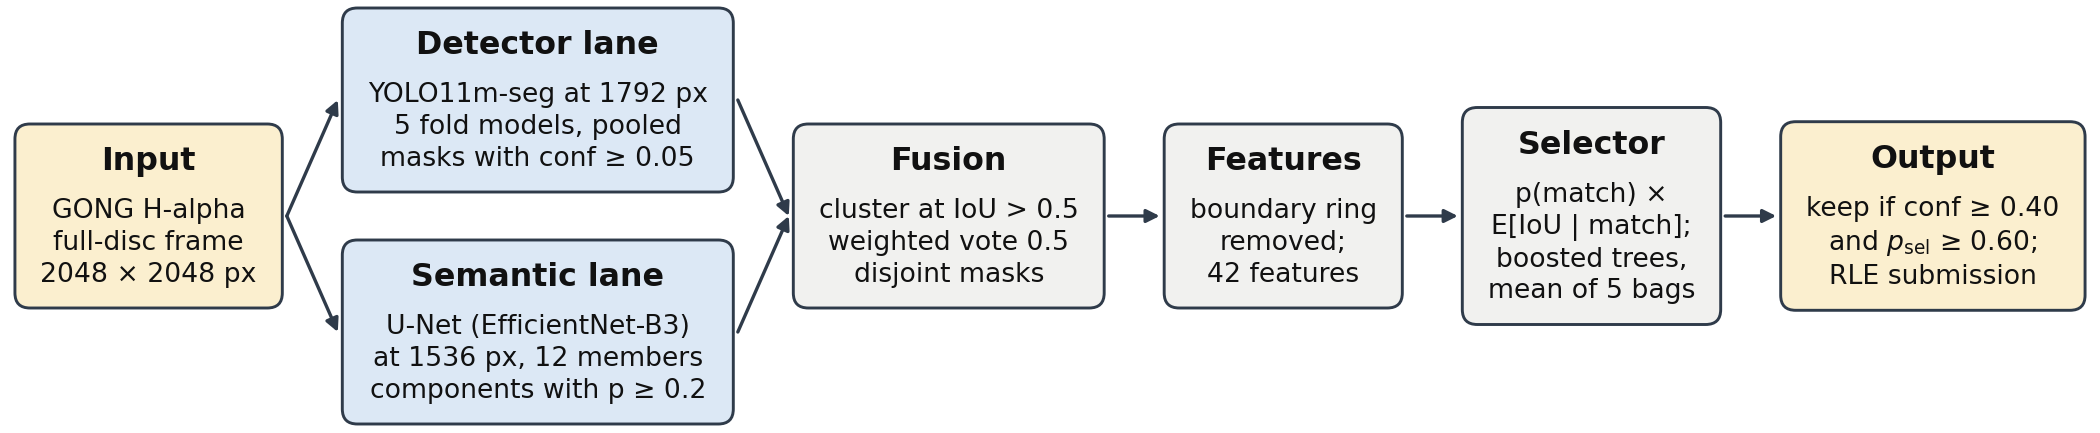
\includegraphics[width=\textwidth]{figures/pipeline.png}
  \caption{Boru hattı. İki hat, örnek adaylarını birbirinden bağımsız önerir; füzyon bunları piksel düzeyinde ayrık tek bir aday havuzuna dönüştürür; öğrenilmiş bir seçici hangi adayların gönderime yazılacağına karar verir.}
  \Description{Girdi görüntüsünden dedektör hattı ve semantik hat üzerinden füzyon, öznitelikler, seçici ve çıktıya giden bir akış şeması.}
  \label{fig:pipeline}
\end{figure*}

\subsection{Veri, bölmeler ve doğrulama protokolü}\label{sec:protocol}
Veri, altı GONG istasyonundan 707 eğitim ve 180 test görüntüsüdür ($2048\times2048$, 8 bit JPEG); 1154 anotatör-görüntü girişinde 8199 poligon etiketi vardır. Güneş diski $(1023.6, 1024.6)$\,px merkezli ve 899.95\,px yarıçaplıdır (887 görüntünün tamamında standart sapma 0.73\,px); bu nedenle geometrik hizalama uygulanmaz.

Ayrı bir tutulan küme yoktur: eğitim görüntüleri, fiziksel görüntüye göre gruplanmış \texttt{GroupKFold} ile beş kata bölünür; böylece bir görüntünün bütün anotatör girişleri aynı kattadır. Atama bir kez donduruldu (\texttt{data/splits/folds\_v1.parquet}) ve her deneyde değiştirilmeden kullanıldı. Öğrenilen her katman çapraz-uydurulmuştur. Bir eğitim görüntüsü için ağ tahminleri yalnızca o görüntüyü görmemiş kat modelinden gelir; seçici dört katta uydurulup beşincisine uygulanır. Semantik hat her anotatör girişiyle eğitilir, çünkü metrik her kopyaya karşı puanlar. Beş dedektör ise görüntü başına tek bir kopyayla, medoid anotatörün kopyasıyla eğitilir; bütün kopyalarla eğitilen bir dedektör daha sonra kat 0'da $+0.0051$ PQ ölçtü, ama üretimdeki dedektörler yeniden eğitilmedi. Test zamanında beş kat modeli bir topluluk olarak çalışır.

\subsection{Ön-işleme}
Görüntüler teslim edildiği gibi kullanılır. Kontrast eşitleme, yoğunluk uyumlama ya da kenar kararması düzeltmesi yoktur. Semantik hat için görüntü bir kez $1536\times1536$'ya yeniden boyutlandırılır, $[0,1]$ aralığına ölçeklenir ve üç kanala kopyalanır. Maskeler alan ortalamasıyla küçültülür ve 0.5'te eşiklenir; bu, etiketli alanın \%98.1'ini korur ve hiçbir örneği silmez. Dedektör, 1792\,px'te Ultralytics girdi hattını kullanır.

\subsection{Dedektör hattı}
COCO ağırlıklarından \cite{lin2014coco} başlatılmış YOLO11m-seg \cite{yolo11}, tek sınıf, kat başına bir model. Tam-disk geometrisini bozan augmentasyonlar (mosaic, mixup, copy-paste, silme, shear, perspektif, dikey çevirme) kapalıdır. Adaylar güven $\geq 0.05$ ile tutulur. NMS, seçicinin eğitildiği kat-dışı adaylarda IoU 0.5, testte 0.05'tir; 0.05, ilk hafta füzyondan önce tek dedektörde yapılan taramanın optimumudur ($+0.0105$ PQ). Uyumsuzluğu sistemi yeniden üretirken bulduk. Füzyondan sonra kazanç kalmaz: kat 0'da o katın kat-dışı seçicisiyle 0.05, 1927 adaydan hiçbiri eşleşme olmayan 188'ini çıkarır ve PQ'yu $+0.0007$ [$-0.0043$, $+0.0055$] değiştirir. 1024--2048\,px girdi boyutlarından iyileştiren sonuncusu 1792'dir; daha büyük gövde ağları fayda sağlamadı.

\subsection{Semantik hat}
ImageNet ile başlatılmış \cite{deng2009imagenet} EfficientNet-B3 kodlayıcılı \cite{tan2019efficientnet} ve scSE kod çözücü dikkatli \cite{roy2018scse} U-Net \cite{ronneberger2015unet}; Segmentation Models PyTorch \cite{smp} ile kurulmuştur. Kayıp BCE + yumuşak Dice + $0.3\cdot$clDice'tır \cite{shit2021cldice}; clDice iskelet örtüşmesini ödüllendirir, çünkü tek piksellik bir kopukluk bir örneği ikiye böler ve PQ bunu iki kez cezalandırır. Üç üye türü eğitilir: (a) temel tarif, kat başına bir model; (b) örnek-dengeli varyant, kat başına bir model, (c)'nin ağır augmentasyonuyla 60 epoch eğitildi; kaybı, 40\,px yarıçap içindeki her bağlı örneği eşit ağırlıklandırır, böylece küçük filamanlar büyükler kadar sayılır; (c) kat-0 bölmesinde, 768 ve 1536\,px'te 60 epoch eğitilmiş, ağır augmentasyonlu iki model. Test zamanı alanı bunların ağırlıklı ortalamasıdır: (b) için 0.50, (a) için 1/6 ve (c)'nin her modeli için 1/6; her üye kendi eğitim boyutunda, yatay çevirme ortalamasıyla çalıştırılır.

\begin{table}[t]
  \caption{Gönderilen sistemin bütün parametreleri.}
  \label{tab:params}
  \small
  \begin{tabular}{@{}p{0.22\columnwidth}p{0.74\columnwidth}@{}}
    \toprule
    Bileşen & Ayar \\
    \midrule
    Dedektör & YOLO11m-seg, 1792\,px, tek sınıf, medoid hedefler, 40 epoch, patience 15, batch 2, optimizer \texttt{auto} (AdamW, lr 0.002, momentum 0.9 olarak çözülür), lrf 0.01, weight decay 5e-4, ısınma 3 epoch \\
    Dedektör augmentasyonu & döndürme $\pm10^\circ$, öteleme 0.05, ölçek 0.10, yatay çevirme 0.5, parlaklık 0.3; diğerleri kapalı \\
    Semantik model & U-Net, EfficientNet-B3, scSE, 1536\,px, batch 2, AdamW lr 3e-4, weight decay 1e-4, OneCycle (pct\_start 0.1), karma hassasiyet, 30 epoch (örnek-dengeli ve ağır üyeler 60) \\
    Semantik kayıp & BCE + Dice + $0.3\cdot$clDice (5 epoch ısınma); örnek-dengeli varyant: yarıçap 40\,px, ağırlık 1.0 \\
    Semantik augmentasyon & yatay çevirme 0.5, disk merkezi etrafında döndürme $\pm10^\circ$, gama 0.8--1.25; örnek-dengeli ve ağır üyeler: çevirmeler, $90^\circ$ döndürmeler, $\pm20^\circ$, istasyona göre kalibre fotometri \\
    Füzyon & semantik eşik 0.2, en küçük alan 256\,px, küme IoU 0.5, oy 0.5, dedektör NMS kat-dışı 0.5, testte 0.05, en çok 300 tespit \\
    Seçici & sınıflandırıcı: 300 iterasyon, lr 0.05, 31 yaprak, en küçük yaprak 25, L2 1.0; regresör: 300 iterasyon, lr 0.06; 5 görüntü-bootstrap kopyası; 10\,042 eğitim adayı \\
    Tutma kuralı & güven $\geq 0.40$ ve $p_\mathrm{sel}\geq 0.60$ \\
    \bottomrule
  \end{tabular}
\end{table}

\subsection{Füzyon ve öznitelikler}
Görüntü başına, dedektör maskeleri (güven $\geq 0.05$, ağırlık merkezi $r/R\leq 0.97$) ve semantik alanın bağlı bileşenleri ($p\geq 0.2$, alan $\geq 256$\,px), $\mathrm{IoU}>0.5$'te union-find ile kümelenir. Her küme, 0.5 eşiğinde güven ağırlıklı piksel oylamasıyla tek maskeye dönüşür ve maskeler, gönderim biçiminin gerektirdiği gibi, güven sırasıyla açgözlü biçimde piksel düzeyinde ayrık hale getirilir. Her aday, eğitimde ve testte kullanılan tek bir ortak fonksiyondan 42 öznitelik alır: geometri (alan, uzanım, iskelet uzunluğu, genişlik), disk üzerindeki konum, semantik destek (olasılık istatistikleri, halka kontrastı), dedektör desteği (model başına güven, uyum, oy sayısı), aday yoğunluğu, ham görüntünün fotometrisi ve yapı-tensörü yönelimi.

\subsection{Seçici ve tutma kuralı}\label{sec:selector}
Seçici iki histogram gradyan-artırma modelidir \cite{pedregosa2011sklearn}: ``bu aday bir anotatör kopyasıyla eşleşir'' sınıflandırıcısı, yalnızca pozitiflerde uydurulmuş ve eşleştiği kopyalar üzerinden toplanan IoU'yu tahmin eden bir regresörle çarpılır. Çarpım, kendi kat-dışı dağılımının kantiline eşlenerek $p_\mathrm{sel}$ skorunu verir. Gönderilen seçici, her biri görüntülerin bootstrap örneğinde uydurulmuş beş böyle çiftin ortalamasıdır. Tutma kuralı Denklem~\ref{eq:pq}'den çıkar: bir aday eklemek, beklenen kopya ağırlıklı IoU toplamı $\tfrac12\,c\,\mathrm{PQ}$'yu aştığında PQ'yu yükseltir; burada $c$ görüntü başına ortalama kopya sayısıdır ve bu değer çalışma noktamızda 0.361'dir. Ölçülen kalibrasyon bu değeri 0.55--0.60 (0.364) ile 0.60--0.65 (0.485) skor bantları arasında keser; bu yüzden tutma kapısı güven $\geq 0.40$ ve $p_\mathrm{sel}\geq 0.60$'tır.

\subsection{Ardıl-işleme ve gönderim}
Öznitelik çıkarımından önce her maske bir piksellik sınır halkasını kaybeder; bu, konturlarımızın anotatörlerinkini içine alma yönündeki ölçülmüş eğilimini düzeltir ($+0.0128$ PQ). 64\,px'ten küçük maskeler atılır, kalanlar run-length kodlamasıyla yazılır. Nihai gönderim 180 görüntünün 177'sinde 1117 örnek içerir (Şekil~\ref{fig:examples}).

\begin{figure*}[t]
  \centering
  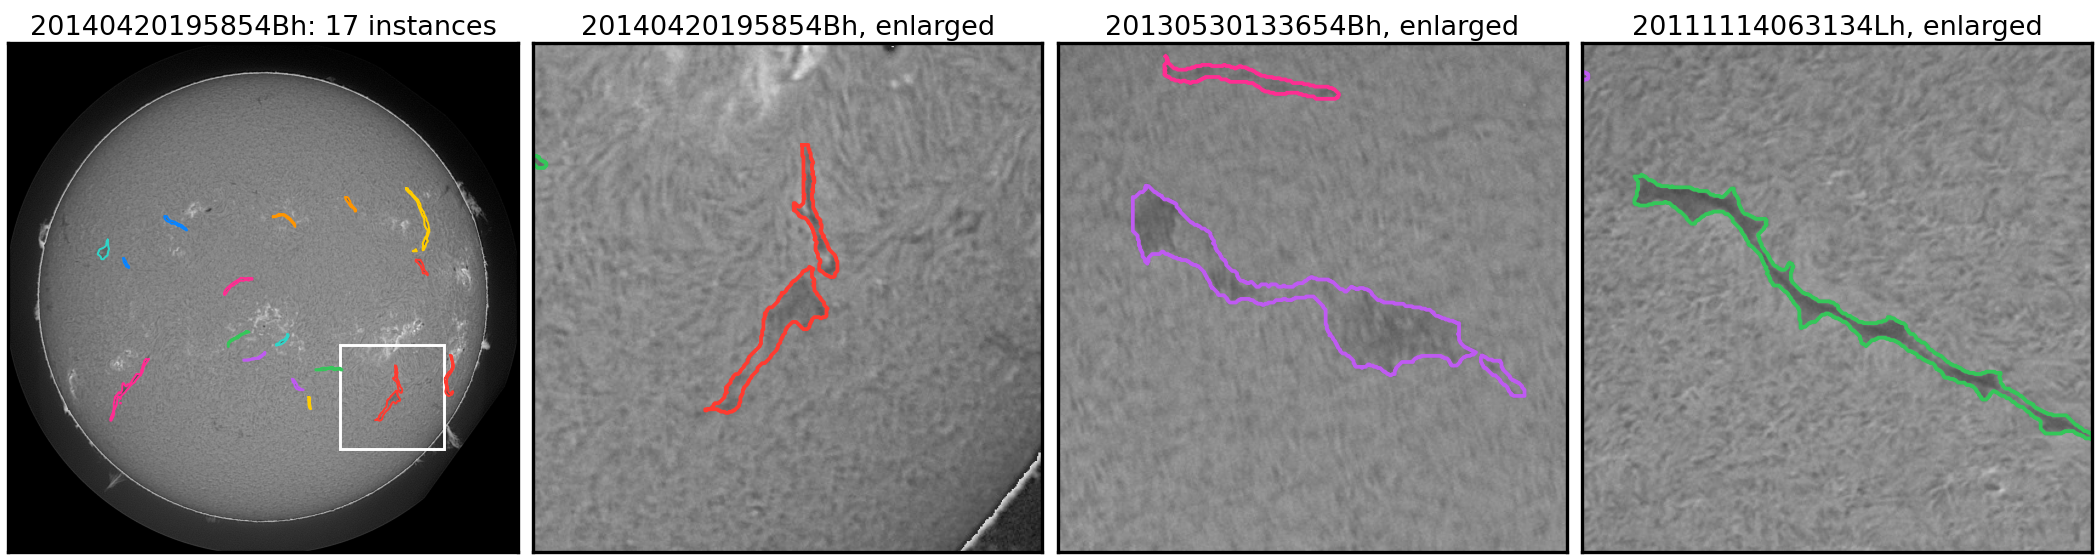
\includegraphics[width=0.78\textwidth]{figures/examples.png}
  \caption{Test görüntülerinde nihai gönderim: tahmin edilen her örneğin konturuyla bir tam-disk görüntü ve bu görüntü ile başka yıllardan iki görüntünün büyütülmüş bölgeleri. Görüntüler kuralla seçilmiştir (en çok tahmin edilen örnek).}
  \Description{Tahmin edilen filamanların renkli konturlarıyla bir tam-disk H-alfa görüntüsü ve konturların koyu, uzun filamanları izlediği üç büyütülmüş bölge.}
  \label{fig:examples}
\end{figure*}

\section{Değerlendirme}\label{sec:evaluation}

\subsection{Strateji}
Bütün skorlar, Denklem~\ref{eq:pq}'in organizatörlerin yayımladığı puanlayıcıyla eşitlik açısından test edilmiş uygulamamızla, beş tutulan kat üzerinden havuzlanmıştır (Bölüm~\ref{sec:protocol}). Aralıklar, görüntüler üzerinde \%95 bootstrap aralıklarıdır (4000 yeniden örnekleme). Bir değişiklik, ancak eşleştirilmiş bootstrap onu önceden kaydedilmiş $\pm0.003$'lük ölçüm tabanının üstüne yerleştirirse benimsenir: tek bir topluluk üyesinin tohum tekrarı PQ'yu $\pm0.001$ oynatır; aynı seçici varyantı beş farklı kat bölüntüsünde 0.0015 standart sapmayla oynar.

\subsection{Sonuçlar}
Tablo~\ref{tab:results}, aynı bileşenlerden kurulan daha basit sistemleri iki insan referansı arasında puanlar: diğerlerine karşı puanlanan tek bir anotatör ve bütün anotatörlerin çizimlerinden kurulan çoğunluk-konsensüs maskesi. Üç referans sistemin eşikleri örnek-içi seçilmiştir; bu onların lehinedir. Semantik hat tek başına dedektörü geçer, ikisini füzyonlamak $+0.021$ ekler, öğrenilmiş seçici $+0.009$ daha ekler ve bunun tamamı kesinliktir: 289 doğru pozitif pahasına 840 yanlış pozitifi kaldırır. Tam sistem için aralıklar PQ $[0.434, 0.452]$, SQ $[0.675, 0.681]$ ve RQ $[0.641, 0.665]$'tir; beş kat sırasıyla 0.451, 0.447, 0.448, 0.458 ve 0.412 okur.

\begin{table}[t]
  \caption{707 eğitim görüntüsünde kat-dışı sonuçlar.}
  \label{tab:results}
  \small\setlength{\tabcolsep}{3.6pt}
  \begin{tabular}{@{}lrrrrrr@{}}
    \toprule
    Sistem & PQ & SQ & RQ & TP & FP & FN \\
    \midrule
    Tek anotatör, diğerlerine karşı & 0.340 & 0.634 & 0.536 & & & \\
    Yalnız dedektör & 0.398 & 0.665 & 0.598 & 4492 & 2339 & 3707 \\
    Yalnız semantik hat & 0.413 & 0.677 & 0.610 & 5273 & 3810 & 2926 \\
    Füzyon, güven kapısı & 0.434 & 0.675 & 0.643 & 5106 & 2569 & 3093 \\
    \textbf{Tam sistem} & \textbf{0.443} & 0.678 & 0.653 & 4817 & 1729 & 3382 \\
    Bütün anotatörlerin konsensüsü & 0.641 & 0.790 & 0.812 & & & \\
    \bottomrule
  \end{tabular}
\end{table}

Eşleşen kopyalarda IoU'nun medyanı 0.683 (çeyrekler 0.615 ve 0.742; 5. ve 95. yüzdelikler 0.533 ve 0.810), Dice'ın medyanı 0.812'dir (çeyrekler 0.762 ve 0.852; 5. ve 95. yüzdelikler 0.695 ve 0.895). Tablo~\ref{tab:relations}, ilişki dağılımlarını organizatörlerin öz-değerlendirme notebook'undaki tanımla verir: parçalanma ve birleşme \%2--3 dolayındadır; eşleşmeyen kütlenin geri kalanı saf kaçırmalar ve saf fazlalıklardır. Bu dağılımlar seçici torbalanmadan önceki noktada okunmuştur (PQ 0.4421); torbalama $+0.0010$ ekler.

\begin{table}[t]
  \caption{Bire-çok (parçalanma) ve çoka-bir (birleşme) ilişkileri, kat-dışı.}
  \label{tab:relations}
  \small
  \begin{tabular}{@{}lrrr@{}}
    \toprule
    Yön & bir & iki veya daha çok & hiç \\
    \midrule
    Yer gerçeği $\rightarrow$ tahminler & \%69.9 & \%2.1 & \%28.0 \\
    Tahminler $\rightarrow$ yer gerçeği & \%87.8 & \%2.6 & \%9.6 \\
    \bottomrule
  \end{tabular}
\end{table}

Açık liderlik tablosu 0.40 gösterir. Yerel tahmine göre $-0.04$ ile $-0.05$ arasındaki fark, boru hattının her neslinde aynıdır. Aynı maskeleri farklı anotatörlere karşı puanlamak PQ'yu $-0.036$ ile $+0.038$ arasında oynatır; bu yüzden farkı test anotatörlerine bağlıyor ve gizli yarıda 0.40--0.42 bekliyoruz. 17 ağın eğitimi yaklaşık 30 GPU-saat sürdü; on beşi kulvarların kat modelleridir ve kat-dışı seçici bunları zaten gerektirir; test yolu tek bir 16\,GB GPU'da 17 dakikada koşar.

\subsection{Güçlü yönler}
Maske kalitesi etiketin tekrarlanabilirliği düzeyindedir: iki anotatörün çizdiği 2483 eşleşen kopyada maskemiz, vakaların \%76.2'sinde bir anotatöre ikinci anotatörden daha yakındır (SQ 0.678, anotatörler arası IoU 0.634). Örnek yapısı temizdir (Tablo~\ref{tab:relations}). Seçici skoru en yüksek on altı yanlış pozitifin hepsi, o görüntünün hiçbir anotatörünün çizmediği, gözle açıkça filaman olan yapılardır; yani yanlış pozitif sayısının bir kısmı gerçek yapının yakalanmasıdır.

\subsection{Zayıf yönler ve iyileştirme stratejileri}
Kalan kayıp tanımadadır: duyarlılık (recall) 0.588, kesinlik 0.736'dır. Disk üzerindeki anotatör kopyalarının \%60.6'sı eşleşir; \%11.5'inde IoU 0.5'in üstünde bir aday vardı ama seçici reddetti; \%3.4'ü hiç önerilmedi; \%24.6'sının IoU'su 0.05 ile 0.5 arasında bir adayı vardır, yani doğru nesne, yanlış şekil. İkinci bir anotatörün doğruladığı böyle kopyalarda adayımız ince değil kısadır (medyan iskelet oranı 0.72, genişlik oranı 1.04) ve bu vakaların \%75'inde eksik kısım üzerinde topluluğun olasılığı neredeyse sıfırdır. Barb'lar aynı sınırı gösterir (Şekil~\ref{fig:barbs}). Barb pikselini, etiketli omurgaya göre, gövdeden ince ve omurgadan yarım gövde genişliğinden uzak piksel olarak tanımlarsak, eşleşen maskelerimiz barb piksellerinin \%38.0'ini kapsar, ikinci bir anotatör \%49.3'ünü; gövdede bu oranlar \%80.5 ve \%79.7'dir. Tanıma kenarda da düşer ($r/R$ 0.8--0.9 için RQ 0.556, disk üzerinde 0.66--0.67); SQ ise 0.68'de kalır.

\begin{figure}[t]
  \centering
  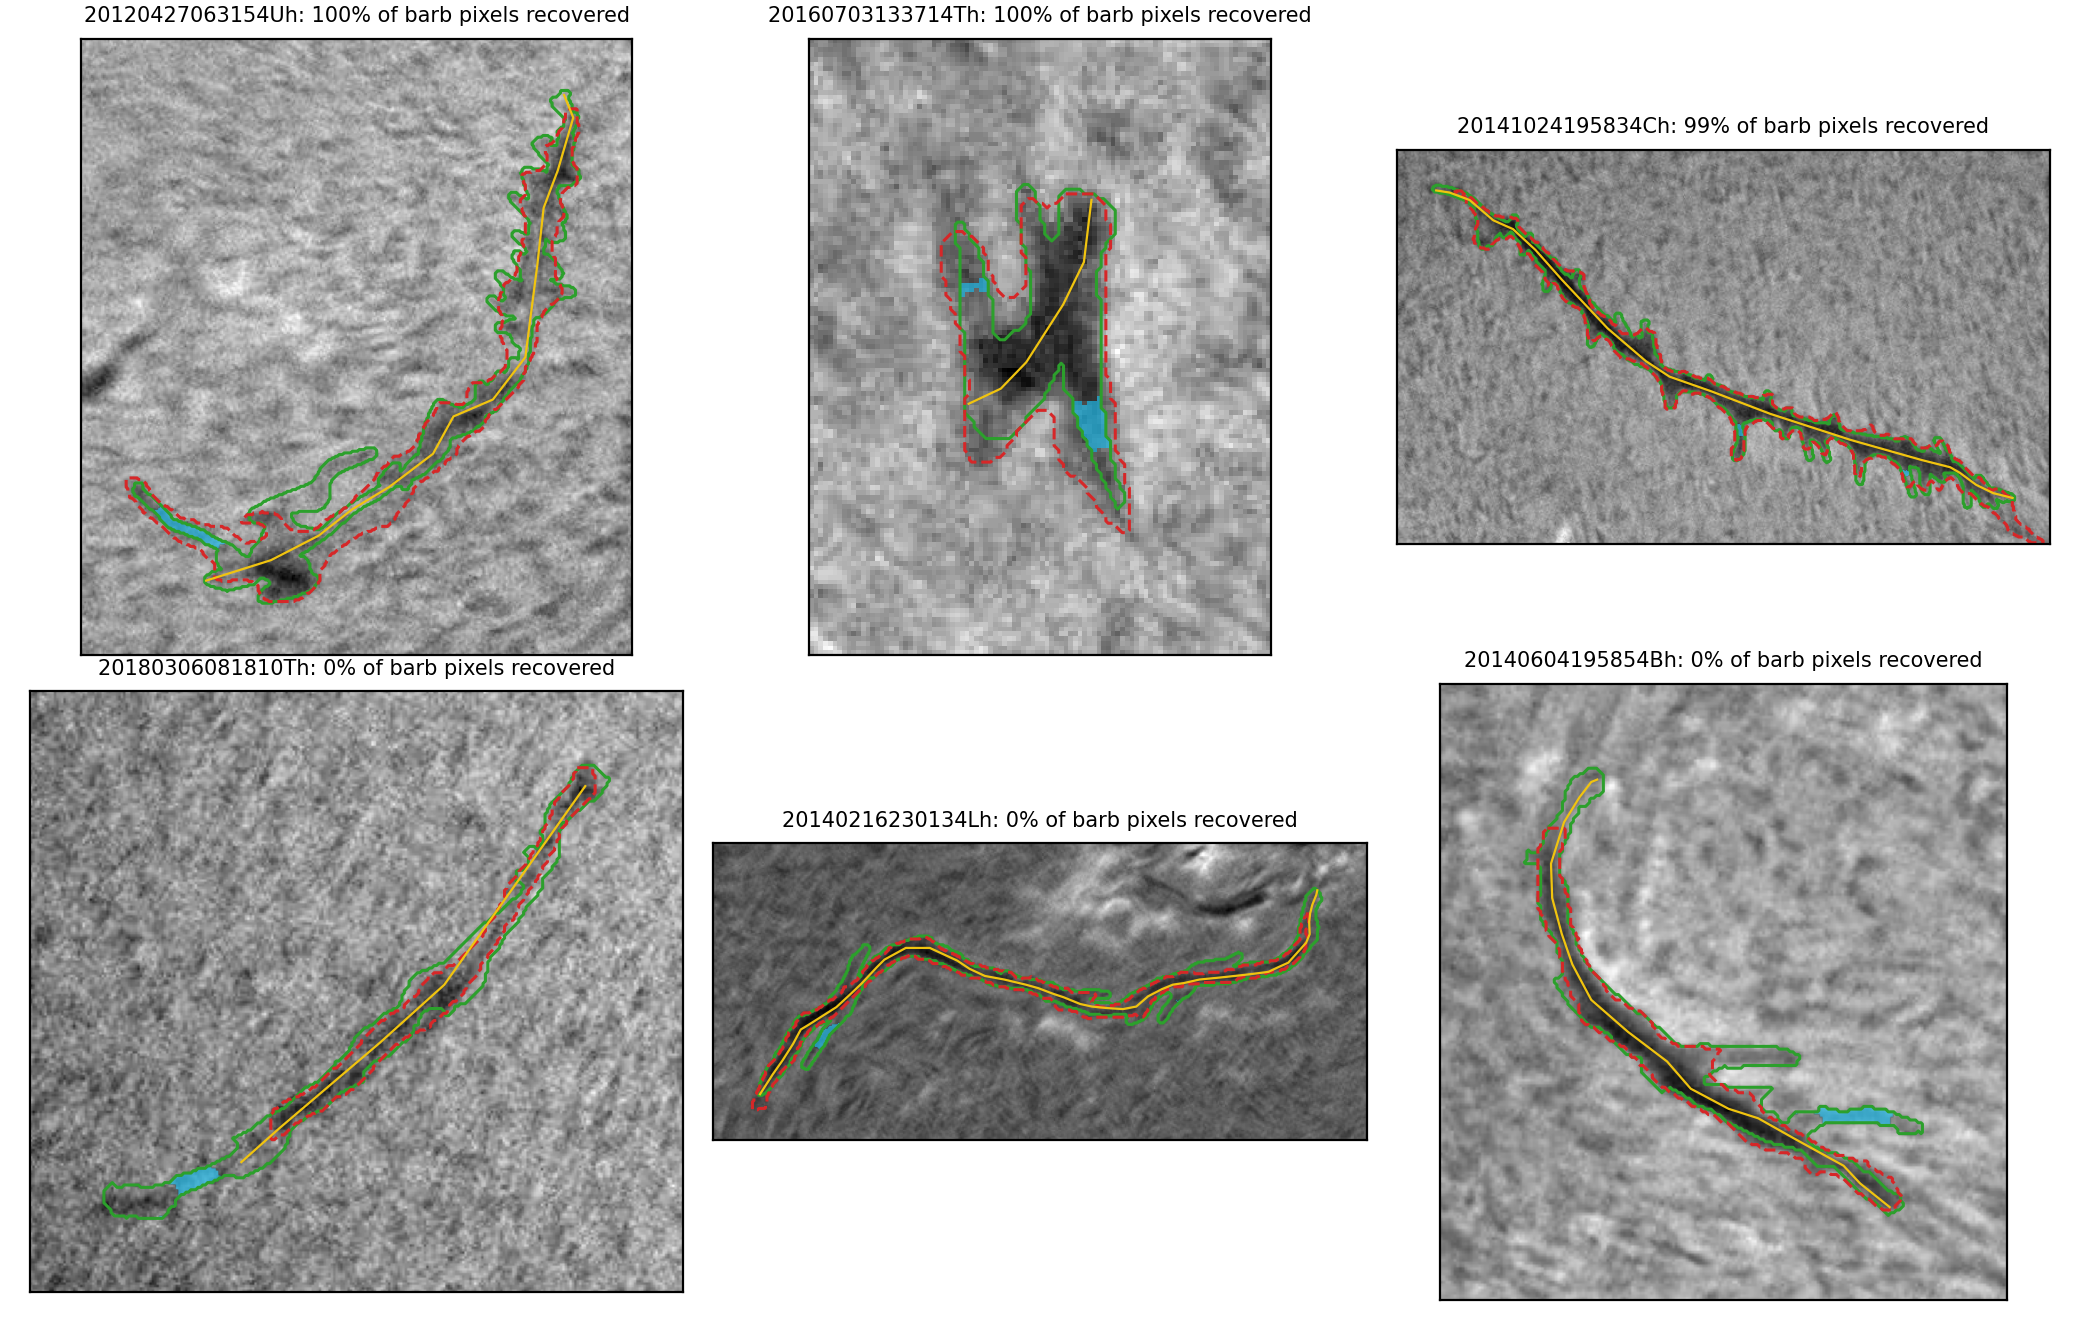
\includegraphics[width=0.70\columnwidth]{figures/barbs.png}
  \caption{Etiketli eğitim filamanlarının barb'ları (taralı); anotatörün konturu (düz), kat-dışı maskemiz (kesikli) ve etiketli omurga. Üst satır: barb'ları en iyi geri kazanılan üç eşleşen kopya; alt satır: en az geri kazanılan üçü.}
  \Description{Anotatör konturları, tahmin konturları ve omurgalarla altı büyütülmüş H-alfa bölgesi; koyu gövdeye bağlı kısa barb'lar izlenir, uzun ve soluk olanlar izlenmez.}
  \label{fig:barbs}
\end{figure}

Tablo~\ref{tab:negative}, aynı protokolle uygulanıp ölçülen ve ölçüm tabanını geçemeyen değişiklikleri listeler. Bunlar sınırı füzyonda, seçimde ya da ardıl-işlemede değil, ağların soluk yapıya verdiği yanıtta konumlandırır: füzyon oyunu birleşime doğru kaydırmak $-0.058$ PQ'ya, maskeleri görüntü yoğunluğuna oturtmak $-0.070$'e mal olur; seçimin görünen payı (havuzu tek bir anotatörün bilgisiyle yeniden sıralamak, $+0.033$) aynı seçim başka bir anotatöre karşı puanlandığında kaybolur. Bu yüzden iki yön görüyoruz. Birincisi, soluk uzunluğu ve barb'ları hedefleyen gözetim; PQ'nun kendisi buna teşvik vermez (barb'lar etiketli alanın \%0.17'sidir). İkincisi, görüntü başına birden çok anotatörlü etiketler: yanlış şekilli kopyaların \%66.5'ini yalnızca bir anotatör çizmiştir ve konsensüs oracle'ı açığın ne kadarının etiket varyansı olduğunu gösterir.

\begin{table}[t]
  \caption{Ölçülen ve $\pm0.003$ ölçüm tabanını geçemeyen değişiklikler.}
  \label{tab:negative}
  \small
  \begin{tabular}{@{}p{0.55\columnwidth}p{0.41\columnwidth}@{}}
    \toprule
    Değişiklik & Ölçülen etki \\
    \midrule
    Dokuz kodlayıcı (13--93\,M parametre), UNet++, UPerNet, SegFormer üye olarak & tohum tekrarının $\pm0.001$ içinde \\
    Üçüncü hat olarak Mask2Former & $+0.0020$ $[-0.0027, +0.0066]$ \\
    Adaya koşullu maske iyileştirici & üç biçimin en iyisi $-0.015$ \\
    Etiketsiz GONG görüntüleriyle ön-eğitim & tohum tekrarına eşit \\
    HMI manyetogramı, öğretmen girdisi olarak & $+0.0015$, $+0.0003$ (iki kat) \\
    Semantik eşik 0.10, seçici yeniden uydurularak & $+0.0010$ $[-0.0019, +0.0038]$ \\
    Görüntü rejimine göre tutma eşiği & $+0.0019$ $[-0.0006, +0.0044]$ \\
    $0.40\leq p_\mathrm{sel}<0.60$ bandında kaskad & $+0.0008$ $[-0.0011, +0.0026]$ \\
    \bottomrule
  \end{tabular}
\end{table}

\section{Yeniden üretilebilirlik ve uyum}\label{sec:repro}
Depo modülerdir (metrik, önbellek kurucular, eğitim ve çıkarım, ölçüm başına bir betik) ve \texttt{requirements.txt} her paketi sürümüyle sabitler. \texttt{notebooks/} altındaki notebook boru hattını üç modda çalıştırır: depodaki test aday havuzundan son aşama (CPU, saniyeler), yayımlanan ağırlıklardan tam çıkarım ya da baştan eğitim. Aday havuzundan, gönderilen dosya bayt bayt yeniden üretilir; seçici depodaki eğitim havuzundan yeniden uydurulduğunda da sonuç bayt bayt aynıdır.

Hiçbir dış etiket kullanılmadı. Gönderilen modellerin tek dış girdileri ImageNet kodlayıcı ağırlıkları ve COCO ile ön-eğitilmiş dedektör ağırlıklarıdır; manyetogramlar ve etiketsiz GONG görüntüleri yalnızca Tablo~\ref{tab:negative}'teki deneylerde yer alır ve çıkarım yalnızca verilen H-$\alpha$ görüntülerini okur. Organizatörlerin izin verdiği biçimde, kodlama ve yazımda yapay zekâ araçları kullanıldı; yukarıdaki her tasarım kararı depodaki kayıtlı bir ölçüme dayanır.

\section{Teşekkür}\label{sec:acknowledgment}
    Filament Segmentation Challenge 2026'nın düzenlenmesi, ABD Ulusal Bilim Vakfı (NSF) tarafından 2209912 ve 2433781 numaralı hibelerle (Computer and Information Science and Engineering direktörlüğü, Office of Advanced Cyberinfrastructure) ve 2511630 numaralı hibeyle (AST Division Of Astronomical Sciences, MPS Directorate for Mathematical and Physical Sciences) kısmen desteklenmektedir.

    Filament Segmentation Challenge 2026'nın sponsoru ABD Ulusal Bilim Vakfı (NSF) Ulusal Güneş Gözlemevi'dir (NSO).

    Bu çalışma, NSO Integrated Synoptic Program tarafından elde edilen GONG verilerini kullanır; program, Ulusal Bilim Vakfı ile yapılan işbirliği anlaşması kapsamında ve National Oceanic and Atmospheric Administration'ın katkısıyla Association of Universities for Research in Astronomy (AURA), Inc. tarafından işletilen National Solar Observatory tarafından yönetilmektedir. GONG gözlem ağına Big Bear Solar Observatory, High Altitude Observatory, Learmonth Solar Observatory, Udaipur Solar Observatory, Instituto de Astrofísica de Canarias ve Cerro Tololo Interamerican Observatory ev sahipliği yapmaktadır.

\bibliographystyle{ACM-Reference-Format}
\bibliography{main}

\end{document}
